% IF YOU CAN SEE THIS GO CONTRIBUTE >:(

\documentclass[letterpaper, 8pt]{extarticle}
\usepackage{amssymb,amsmath,amsthm,amsfonts}
\usepackage{multicol,multirow}
\usepackage{calc}
\usepackage{ifthen}
\usepackage[landscape]{geometry}
\usepackage[colorlinks=true,citecolor=blue,linkcolor=blue]{hyperref}

\usepackage{booktabs}
\usepackage{ulem}
\usepackage{enumitem}
\usepackage{tabulary}
\usepackage{graphicx}
\usepackage{siunitx}
\usepackage{tikz}
\usepackage{derivative}
\usepackage{svg}
\usepackage{listings}
\usepackage{setspace}
\usepackage{listings}
\usepackage{xcolor}
\usepackage{courier}
\usepackage{syntax}
\usepackage{mathpartir}

% minimal line spacing
\setstretch{0.1}

% set borders (experimentally determined to minimize cutoff and maximize space on school printers)
\geometry{top=.25in,left=.25in,right=.25in,bottom=.35in}

% make figures work better in multicol
\newenvironment{Figure}
{\par\medskip\noindent\minipage}
{\endminipage\par\medskip}

\pagestyle{empty} % clear page

% rewrite section commands to be smaller
\makeatletter
\renewcommand{\section}{\@startsection{section}{1}{0mm}%
                                {-1explus -.5ex minus -.2ex}%
                                {0.5ex plus .2ex}%x
                                {\normalfont\normalsize\bfseries}}
\renewcommand{\subsection}{\@startsection{subsection}{2}{0mm}%
                                {-1explus -.5ex minus -.2ex}%
                                {0.5ex plus .2ex}%
                                {\normalfont\small\bfseries}}
\renewcommand{\subsubsection}{\@startsection{subsubsection}{3}{0mm}%
                                {-1ex plus -.5ex minus -.2ex}%
                                {1ex plus .2ex}%
                                {\normalfont\tiny\bfseries}}
\makeatother
\setcounter{secnumdepth}{0} % disable section numbering


% disable indenting
\setlength{\parindent}{0pt}
\setlength{\parskip}{0pt plus 0.5ex}

% Custom siunitx defs
\DeclareSIUnit\noop{\relax}
\NewDocumentCommand\prefixvalue{m}{%
\qty[prefix-mode=extract-exponent,print-unity-mantissa=false]{1}{#1\noop}
}

% Shorthand definitions
\newcommand{\To}{\Rightarrow}
\newcommand{\ttt}{\texttt}
\newcommand{\ra}{\rightarrow}

% condense itemize & enumerate
\let\olditemize=\itemize \let\endolditemize=\enditemize \renewenvironment{itemize}{\olditemize \itemsep0em}{\endolditemize}
\let\oldenumerate=\enumerate \let\endoldenumerate=\endenumerate \renewenvironment{enumerate}{\oldenumerate \itemsep0em}{\endoldenumerate}
\setlist[itemize]{noitemsep, topsep=0pt, leftmargin=*}
\setlist[enumerate]{noitemsep, topsep=0pt, leftmargin=*}

\title{3N03}

\begin{document}
\raggedright
\tiny

% make listings look nicer
\lstset{
	tabsize = 2, %% set tab space width
	showstringspaces = false, %% prevent space marking in strings, string is defined as the text that is generally printed directly to the console
	basicstyle = \tiny\ttfamily, %% set listing font and size
	breaklines = true, %% enable line breaking
	numberstyle = \tiny,
	postbreak = \mbox{\textcolor{red}{\(\hookrightarrow\)}\space}
}

\begin{center}
	{\textbf{3N03 Final Cheatsheet}} \\
\end{center}
% set column spacing rules
\setlength{\premulticols}{1pt}
\setlength{\postmulticols}{1pt}
\setlength{\multicolsep}{1pt}
\setlength{\columnsep}{2pt}
\begin{multicols*}{4}

	\section{Network Fundamentals}
	\textbf{Network:} Collection of devices interconnected by a single technology (internet) \\
	\subsection{Network Uses}
	\textbf{Business Applications:} Resource/info sharing, communication, client-server model \\
	\textbf{Home Applications:} Peer-to-peer model \\
	\textbf{Mobile Users:} Wireless connectivity

	\subsection{E-Commerce Types}
	B2C: Business to Consumer \\
	B2B: Business to Business \\
	G2C: Government to Consumer \\
	C2C: Consumer to Consumer \\
	P2P: Peer to Peer

	\subsection{Social Issues}
	Network Neutrality, Content ownership, Anonymity \& Censorship, Privacy, Info Theft

	\subsection{Network Scales}
	\textbf{PAN:} Personal (Bluetooth) \\
	\textbf{LAN:} Local (Office) \\
	\textbf{MAN:} Metropolitan (City) \\
	\textbf{WAN:} Wide (Country/ISP (Internet Service Provider), a company). Serve as modern internet backbone. \\
	\textbf{Internet:} Network of networks (Planet)
	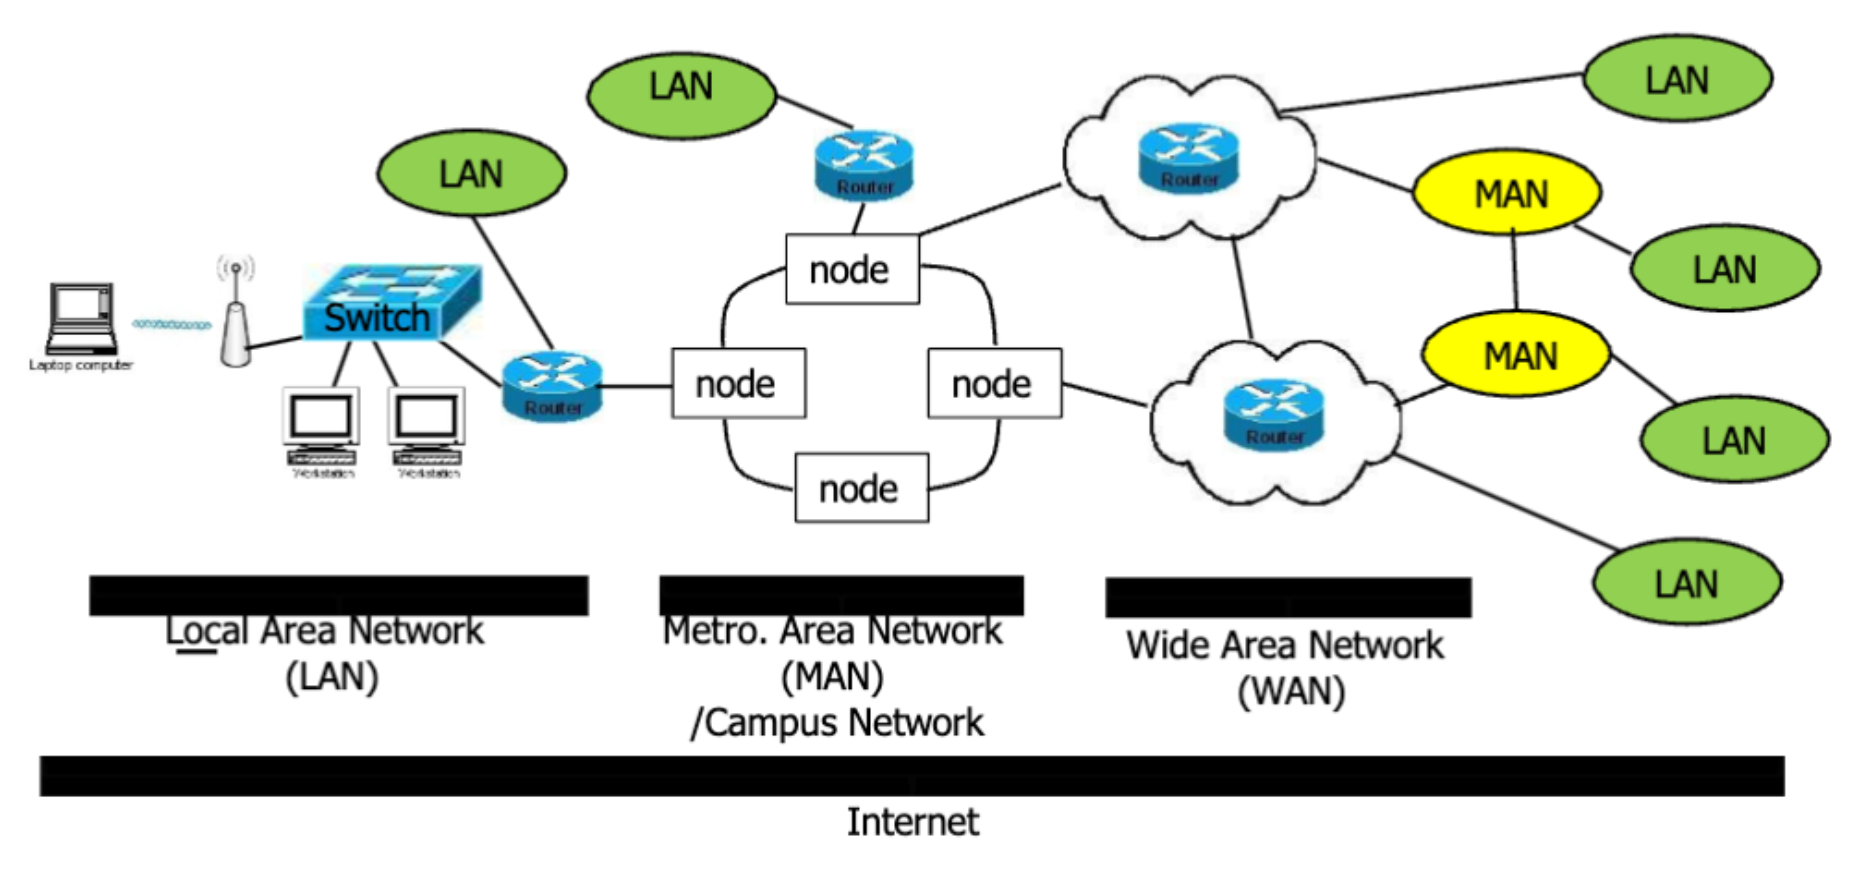
\includegraphics[width=\linewidth]{SCR-20250416-trqu.png}

	\subsection{Connection Types}
	\textbf{Internetwork:} Network of smaller networks \\
	\textbf{Internet:} Set of all connected networks \\
	\textbf{Gateway:} Device transferring data between layers \\
	\textbf{Low-Level Gateways:}
	\begin{itemize}
		\item Operate at the lower layers of the network protocol
		\item More limited in functionality
		\item Cannot effectively connect different types of networks
		\item *Focus on basic data transmission*
	\end{itemize}
	\textbf{High-Level Gateways:}
	\begin{itemize}
		\item Operate at higher layers of the protocol stack (application layer)
		\item Very specific in their function
		\item Limited to particular applications or services
		\item Example: An email gateway that only handles email traffic
		\item *While powerful for specific uses, they're too specialized for general network connectivity*
	\end{itemize}
	\textbf{Best Mid-level Gateways}
	\begin{itemize}
		\item "just right"
		\item Represented by routers, which operate at the network layer
		\item Provide the optimal balance between functionality and flexibility
		\item Can effectively route packets between different networks
		\item \textit{Handle most common networking needs}
		\item Can connect different types of networks while maintaining good performance
	\end{itemize}
	\textbf{Router:} Gateway for network layer information

	\subsection{Transmission Technology}
	\begin{itemize}
		\item broadcast links - communication channel shared by all machines in network
		\item point-to-point - direct connection between two machines
		\item packet - small unit of data sent over a network.
	\end{itemize}

	\section{Layered Network Models}
	Each layer implements a service. Layering provides encapsulation, where each layer adds its own header to data.

	\subsection{Design Issues}
	\begin{itemize}
		\item Reliability/failure handling
		\item Network growth capability
		\item Resource allocation
		\item Security against threats
	\end{itemize}

	\subsection{Layer services}
	\textbf{Vertical:} services for uni directional communication from top layer to bottom layer, like a gateway \\
	\textbf{Horizontal:} protocols for communication between same layers
	\textbf{connection oriented:} set up for ongoing use, torn down afterwords
	\textbf{connectionless:} separately and temporary handled messages

	\subsection{OSI Model}
	Open Systems Interconnection. Makes essential concepts explicit (services, interfaces, protocols). \\
	\textbf{7. Application:} Network apps, end-user access, protocols (FTP, SMTP, HTTP) \\
	\textbf{6. Presentation:} Data interpretation/formatting \\
	\textbf{5. Session:} provides locality for different transport streams to not confuse individual streams. Estabashing a method of communicatino. \\
	\textbf{4. Transport:} Process-to-process data transfer, segmentation, reliability (TCP, UDP) \\
	\textbf{3. Network:} packet routing between networks (IP) \\
	\textbf{2. Data Link:} raw bit collection, physical addressing, unit of data in frames \\
	\textbf{1. Physical:} Raw bit transmission (cables, signals)
	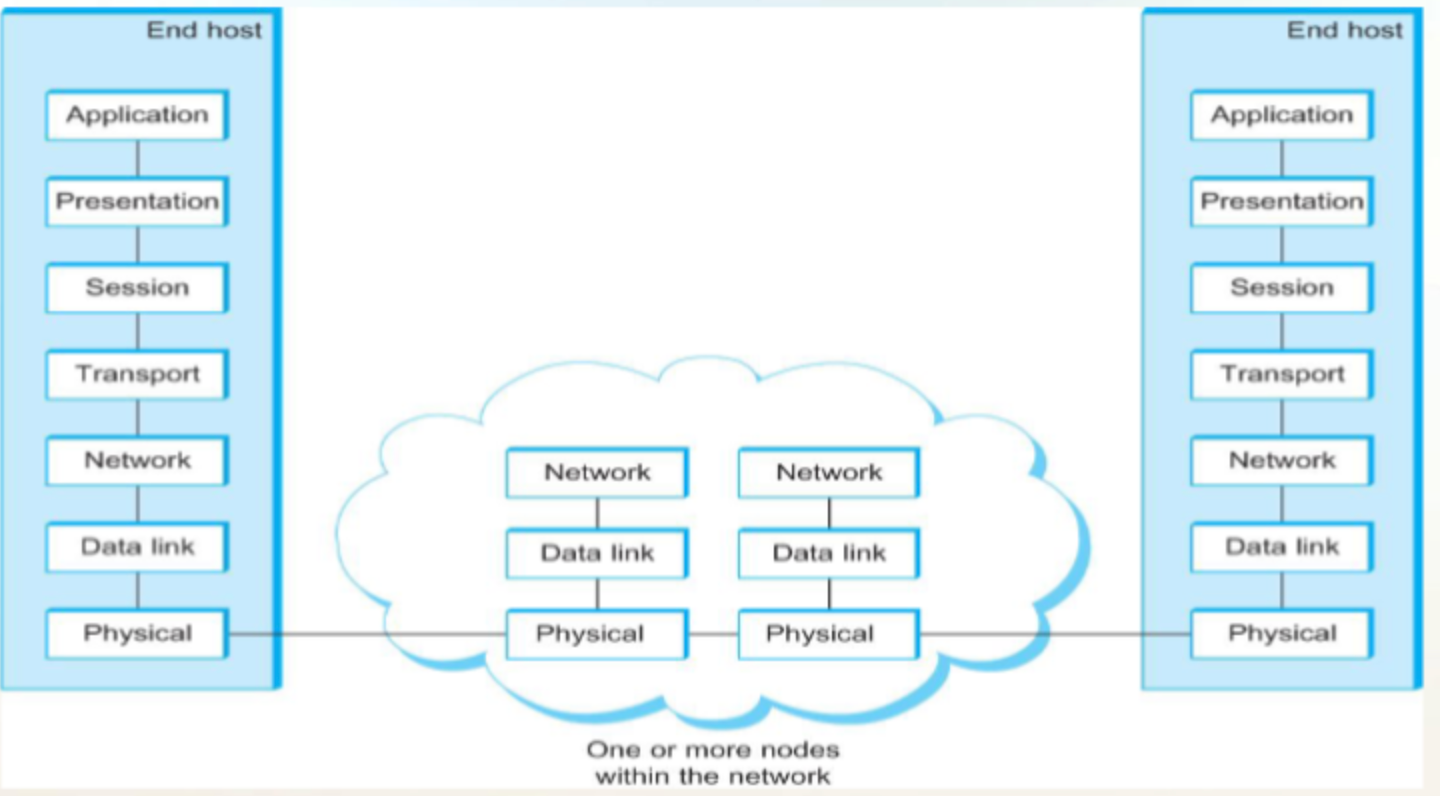
\includegraphics[width=\linewidth]{SCR-20250416-ucdl.png}

	\subsection{TCP/IP Model}
	More specific to the internet, heavily relies on protocols, whereas OSI model is more generalized. \\
	\textbf{4. Application:} TELNET, FTP, SMTP, DNS, HTTP, RTP \\
	\textbf{3. Transport:} TCP (reliable, connection-oriented), UDP (unreliable, connectionless) \\
	\textbf{2. Internet:} IP packet delivery, multi-network connection support. \\
	\textbf{1. Link:} implemented by combinatino of hardware (ethernet, fiberoptics, etc).
	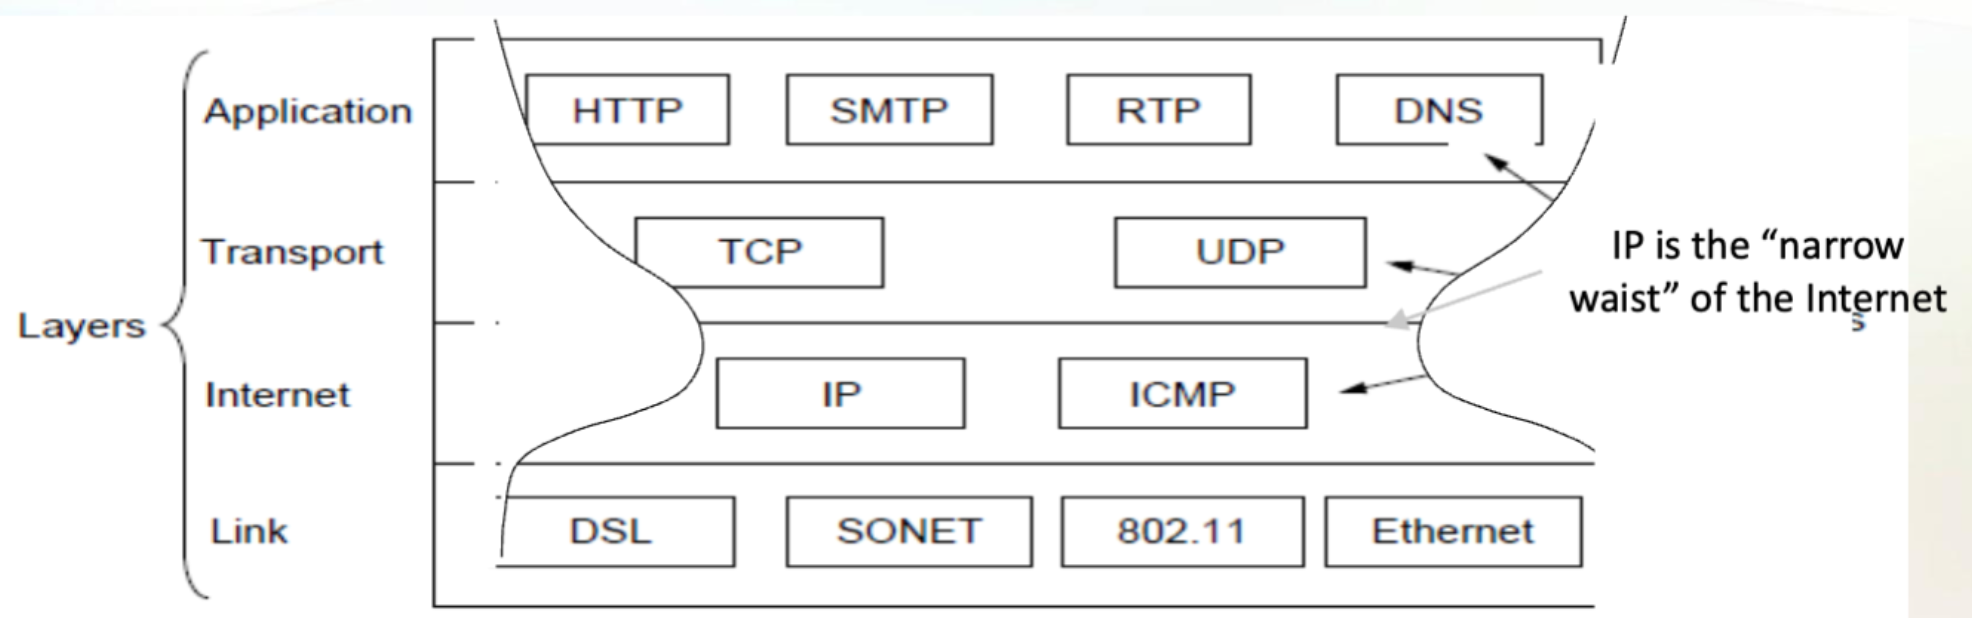
\includegraphics[width=\linewidth]{SCR-20250416-udrs.png}

	\section{Data Transmission}
	\textbf{Packet Transmission Delay:} $\frac{L}{R}$ (Length/Rate) \\
	\textbf{Store \& Forward:} Full packet received before forwarding, end-to-end delay = $2\frac{L}{R}$

	\subsection{Network Core Functions}
	\textbf{Routing:} Determining packet paths \\
	\textbf{Forwarding:} Moving packets between router interfaces

	\section{Application Layer}
	\subsection{Architectures}
	\textbf{Client-Server:}
	\begin{itemize}
		\item Clients communicate with server
		\item Server: permanent IP, always-on
		\item Clients: dynamic IP, intermittent connectivity
	\end{itemize}

	\textbf{Peer-to-Peer (P2P):}
	\begin{itemize}
		\item Minimal server reliance
		\item Direct end-system communication
		\item Self-scaling with new peers
		\item Challenges: security, performance, management
	\end{itemize}

	\subsection{Application Requirements}
	\textbf{Data Transfer:} Reliability needs \\
	\textbf{Timing:} Delay sensitivity \\
	\textbf{Throughput:} Bandwidth requirements \\
	\textbf{Security:} Encryption, authentication

	\subsection{Transport Protocols}
	A protocol is a set of rules governing the format and meaning of the packets or messages that are exchanged. Protocols implement the services.
	\textbf{TCP Service:}
	\begin{itemize}
		\item Reliable transport
		\item Flow control
		\item Congestion control
		\item Connection-oriented
		\item No timing/throughput guarantees
		\item No built-in security
	\end{itemize}

	\textbf{UDP Service:}
	\begin{itemize}
		\item Unreliable data transfer
		\item No guarantees
		\item Low overhead
	\end{itemize}

	\textbf{Securing TCP:} SSL (Secure Socket Layer) at application layer

	\subsection{HTTP Protocol}
	\textbf{Properties:}
	\begin{itemize}
		\item Client/server model
		\item TCP on port 80
		\item Stateless
		\item Non-Persistent: One object per connection
		\item Persistent: Multiple objects per connection
	\end{itemize}

	\textbf{Request Message:}
	\begin{itemize}
		\item ASCII format
		\item Request line, header lines, empty body
	\end{itemize}

	\textbf{Response Message:}
	\begin{itemize}
		\item ASCII format
		\item Status line, header lines, data
	\end{itemize}

	\textbf{Status Codes:}
	\begin{itemize}
		\item 1xx: Informational
		\item 2xx: Success (200 OK)
		\item 3xx: Redirection (301 Moved)
		\item 4xx: Client Error (404 Not Found)
		\item 5xx: Server Error
	\end{itemize}

	\subsection{Cookies}
	Maintain state despite stateless HTTP: response header, request header, browser cookie file, backend database

	\subsection{Web Cache/Proxy}
	Browser connects to proxy not web server; reduces latency, proxy acts as client+server

	\subsection{Email Architecture}
	\textbf{Components:}
	\begin{itemize}
		\item User Agents: Mail clients (Outlook, Apple Mail)
		\item Mail Servers: Mailbox and message queue
	\end{itemize}

	\textbf{SMTP (Simple Mail Transfer Protocol):}
	\begin{itemize}
		\item Client-server between mail servers
		\item Persistent TCP (port 25)
		\item Phases: Handshake, Transfer, Closure
		\item "Push" protocol (sending)
	\end{itemize}

	\textbf{Mail Access Protocols:}
	\begin{itemize}
		\item POP3: Download from server (port 110)
		      \begin{itemize}
			      \item Authorization, Transaction, Update
			      \item Download-and-Delete or Download-and-Keep
			      \item Stateless across sessions
			      \item No remote folders
		      \end{itemize}
		\item IMAP: Remote management on server
		\item HTTP: Web-based email (Gmail, Outlook Web)
	\end{itemize}

	\subsection{DNS (Domain Name System)}
	\textbf{Functions:}
	\begin{itemize}
		\item Hostname/IP translation
		\item Host/Mail server aliasing
		\item Load distribution
		\item Distributed database
		\item Uses UDP (port 53)
	\end{itemize}

	\textbf{Hierarchy:}
	\begin{itemize}
		\item Root DNS servers (13 logical servers)
		\item TLD DNS servers (.com, .org, etc.)
		\item Authoritative DNS servers (organization specific)
		\item Local DNS servers (ISP caching)
	\end{itemize}

	\textbf{Record Types:}
	\begin{itemize}
		\item A: hostname to IP
		\item MX: mail server
	\end{itemize}

	\textbf{Vulnerabilities:}
	\begin{itemize}
		\item DDoS attacks
		\item Redirect attacks (MITM, poisoning)
		\item Using DNS for DDoS amplification
	\end{itemize}

	\section{Transport Layer}
	\textbf{Functions:}
	\begin{itemize}
		\item Logical communication between processes
		\item Implemented in end systems (not routers)
		\item Segments application messages
	\end{itemize}

	\subsection{Internet Protocol Stack}
	\textbf{Network Layer (IP):}
	\begin{itemize}
		\item Host-to-host communication
		\item Best-effort delivery (unreliable)
		\item No guarantees on delivery, order, or integrity
	\end{itemize}

	\subsection{Multiplexing/Demultiplexing}
	\textbf{Process:}
	\begin{itemize}
		\item Transport layer assigns ports
		\item Headers identify destination socket
	\end{itemize}

	\textbf{Identification:}
	\begin{itemize}
		\item TCP sockets: (source IP, source port, dest IP, dest port)
		\item UDP sockets: (dest IP, dest port)
	\end{itemize}

	\textbf{Port ranges:} 0-1023 reserved, 0-65535 total

	\subsection{Reliable Data Transfer}
	\textbf{Error types:}
	\begin{itemize}
		\item Corruption (packet received incorrectly)
		\item Loss (packet never arrives)
	\end{itemize}

	\subsection{UDP Characteristics}
	\textbf{Features:}
	\begin{itemize}
		\item Connectionless
		\item No handshaking
		\item Each segment handled independently
		\item No congestion control
		\item Has checksum for error detection
	\end{itemize}

	\subsection{TCP Characteristics}
	\textbf{Features:}
	\begin{itemize}
		\item Full-duplex service
		\item Point-to-point (single sender, single receiver)
		\item Connection-oriented with handshaking
		\item Reliable, ordered byte stream
		\item Flow control
		\item Congestion control
	\end{itemize}

	\textbf{Segment Structure:}
	\begin{itemize}
		\item Data field (limited by MSS)
		\item 32-bit sequence number
		\item 32-bit acknowledgment number
		\item 16-bit receive window
		\item 4-bit header length
		\item 6-bit flag field
		\item Options field
	\end{itemize}

	\section{Socket Programming}
	\textbf{Socket:} Interface between application and transport protocol

	\textbf{UDP Socket Programming:}
	\begin{itemize}
		\item No connection required
		\item Client attaches destination IP/port
	\end{itemize}

	\textbf{TCP Socket Programming:}
	\begin{itemize}
		\item Connection required
		\item Server needs welcome socket
		\item Creates new socket per client
	\end{itemize}

	\section{Network Layer}
	\subsection{Functions}
	\textbf{Routing:} Network-wide path determination (seconds) \\
	\textbf{Forwarding:} Router-local packet movement (nanoseconds)

	\subsection{Service Models}
	\textbf{Potential Properties:}
	\begin{itemize}
		\item Guaranteed delivery
		\item Bounded delay
		\item In-order delivery
		\item Minimum bandwidth
		\item Security
	\end{itemize}

	\subsection{Router Components}
	\textbf{Input Ports:} Link-layer functions (hardware) \\
	\textbf{Switching Fabric:} Connects ports (hardware) \\
	\textbf{Output Ports:} Transmits packets (hardware) \\
	\textbf{Routing Processor:} Control plane (software)

	\subsection{IP Addressing}
	\textbf{Characteristics:}
	\begin{itemize}
		\item IPv4: 32-bit identifier
		\item IPv6: 128-bit identifier
		\item Assigned by ICANN
		\item Hierarchical: network ID + host ID
	\end{itemize}

	\textbf{Interface:} Connection between host/router and link \\
	\textbf{Network ID:} IP with host ID all zeros \\
	\textbf{Prefix:} Lowest IP in block + size (bits in network portion)

	\subsection{IP Support Protocols}
	\textbf{ICMP:} Error reporting (required) \\
	\textbf{ARP:} Finds MAC for local IP \\
	\textbf{DHCP:} Dynamic IP assignment

	\subsection{IPv6}
	\textbf{Format:} 3fff:0000:0000:0000:0123:4567:89AB:CDEF \\
	\textbf{Shortened:} 3fff::123:4567:89AB:CDEF \\
	\textbf{IPv4 in IPv6:} ::192.31.20.49

	\textbf{Address Types:}
	\begin{itemize}
		\item Unicast: Single interface
		\item Anycast: Set of interfaces (closest)
		\item Multicast: Group of interfaces (all)
	\end{itemize}

	\section{Link Layer}
	\subsection{Functions}
	\begin{itemize}
		\item Encapsulates network datagrams in frames
		\item Error detection/correction
		\item Link access control
		\item Reliable delivery (optional)
	\end{itemize}

	\textbf{Implementation:} Hardware (NIC) + software

	\subsection{MAC Addresses}
	\begin{itemize}
		\item 48-bit (6 bytes)
		\item IEEE managed
		\item Typically permanent (can be spoofed)
	\end{itemize}

	\subsection{ARP Protocol}
	Translates IP addresses to MAC addresses

	\subsection{Ethernet}
	\textbf{Topologies:}
	\begin{itemize}
		\item Bus: Shared collision domain (old)
		\item Switched: Star topology with switch (current)
	\end{itemize}

	\textbf{Frame Structure:}
	\begin{itemize}
		\item Addresses: 6B source, 6B destination
		\item Type field
		\item CRC error checking
		\item Preamble (7B synchronization)
	\end{itemize}

	\textbf{Properties:} Connectionless, unreliable

	\subsection{Switch}
	\begin{itemize}
		\item Stores/forwards frames
		\item Transparent to hosts
		\item Self-learning (no configuration)
		\item Maintains switch table (MAC to interface)
	\end{itemize}

	\section{Physical Layer}
	\subsection{Signal Modulation}
	\textbf{Digital Modulation:} Converting bits to signals

	\textbf{Transmission Types:}
	\begin{itemize}
		\item Baseband: Frequencies from zero up (wires)
		\item Passband: Band around carrier frequency (wireless)
	\end{itemize}

	\subsection{Encoding Methods}
	\textbf{NRZ:} Positive voltage (1), negative voltage (0) \\
	\textbf{Manchester:} XOR with clock, transition direction indicates bit \\
	\textbf{NRZI:} Transition (1), no transition (0) \\
	\textbf{4B/5B:} Limits consecutive same bits

	\subsection{Passband Modulation}
	\textbf{ASK:} Amplitude shift keying (different amplitudes) \\
	\textbf{FSK:} Frequency shift keying (different frequencies) \\
	\textbf{PSK:} Phase shift keying (different phases)

	\subsection{Multiplexing}
	\textbf{TDM:} Time division multiplexing (users take turns) \\
	\textbf{FDM:} Frequency division multiplexing (different bands)

	\subsection{Transmission Media}
	\textbf{Guided Media:}
	\begin{itemize}
		\item Twisted Pair:
		      \begin{itemize}
			      \item Cat 5: 100Mbps (2 pairs)
			      \item Cat 5e: 1Gbps (4 pairs)
			      \item Cat 6: 10Gbps (up to 100m)
			      \item Cat 7: Shielded twisted pair
		      \end{itemize}
		\item Coaxial Cable: Better shielding, high bandwidth
		\item Power Lines: Convenient but noisy
		\item Fiber Optic: Light pulses, low error, high data rate
		      \begin{itemize}
			      \item Single-mode: Narrow, laser, long distance
			      \item Multi-mode: Wider, LED, shorter distance
		      \end{itemize}
	\end{itemize}

	\textbf{Unguided Media:}
	\begin{itemize}
		\item Terrestrial wireless
		\item Satellite
		\item Laser through air
	\end{itemize}

	\subsection{Network Topologies}
	\textbf{Bus:} Single line, simple, one sender at a time \\
	\textbf{Star:} Central switch, more cabling, higher reliability \\
	\textbf{Ring:} Closed loop, token passing, difficult to expand

	\subsection{Network Hardware}
	\textbf{NIC:} Network adapter with MAC address \\
	\textbf{Hub:} All nodes receive transmissions (insecure) \\
	\textbf{Switch:} Only intended recipients receive data \\
	\textbf{Router:} Connects LANs via IP addresses \\
	\textbf{Gateway:} Connects dissimilar networks

	\subsection{Wave Properties}
	\textbf{Frequency (f):} Oscillations per second (Hz) \\
	\textbf{Period (T):} Time between maxima (sec), T = 1/f \\
	\textbf{Wavelength ($\lambda$):} Distance between maxima (m) \\
	\textbf{Relationship:} $\lambda = c/f, c \approx 3 \times 10 m/s$

	\section{Wireless Networks}
	\subsection{Types}
	\textbf{Wireless LANs:} 100ft range, WiFi (54/300/1000 Mbps) \\
	\textbf{Wide-area Wireless:} Cellular, 10's km, 1-100 Mbps

	\subsection{Characteristics}
	\textbf{Advantages:} Easy deployment, mobility support, broadcast capability \\
	\textbf{Challenges:} Interference, variable signal strength/data rates

	\section{Network Security}
	\subsection{Security Properties}
	\textbf{Confidentiality:} Only sender/receiver understand content \\
	\textbf{Message Integrity:} Content unaltered in transit \\
	\textbf{Authentication:} Verify sender/receiver identity \\
	\textbf{Operational Security:} Network protection

	\subsection{Security Concepts}
	\textbf{Firewall:} Controls access between networks \\
	\textbf{Eavesdropping:} Intercepting messages \\
	\textbf{Encryption:} Disguising data from intruders

	\textbf{Key Types:}
	\begin{itemize}
		\item Private/Symmetric: Same key for encrypt/decrypt
		\item Public/Asymmetric: Separate public/private keys
	\end{itemize}

	\subsection{Cryptographic Hash}
	Fixed-size output that's computationally infeasible to reverse or find collisions

	\textbf{Message Authentication:}
	\begin{itemize}
		\item Calculate H(m+s) where s is shared secret
		\item MAC = H(m+s)
		\item Send (m, MAC)
		\item Recipient verifies MAC
	\end{itemize}

	\subsection{Digital Signatures}
	Attests to document agreement

	\subsection{Security Layers}
	Network layer security provides blanket coverage but not user-level security

	\subsection{Network Threats}
	\textbf{Malware Types:}
	\begin{itemize}
		\item Virus: Self-replicating, needs activation
		\item Worm: Self-replicating, auto-spreads
		\item Spyware: Monitors users
		\item Adware: Unwanted advertisements
		\item Scareware: Fake security warnings
		\item Trojan: Hidden malicious function
		\item Ransomware: Encrypts data for ransom
	\end{itemize}

	\subsection{Attack Types}
	\textbf{Reconnaissance (Passive):}
	\begin{itemize}
		\item Ping Sweep: Identifies network hosts
		\item Port Scanning: Discovers services
		\item Packet Sniffing: Captures network data
	\end{itemize}

	\textbf{Access Attacks:}
	\begin{itemize}
		\item Phishing: Fake emails/websites
		\item Pharming: Traffic redirection
		\item MITM: Intercepting connections
		      \begin{itemize}
			      \item Spoofing: False source addressing
			      \item Hijacking: Session takeover
		      \end{itemize}
	\end{itemize}

	\textbf{DoS Attacks:}
	\begin{itemize}
		\item Saturation: Request flooding
		\item Vulnerability exploitation
	\end{itemize}

	\textbf{DDoS:}
	\begin{itemize}
		\item SYN flood: Incomplete TCP handshakes
		\item ICMP flood: Fake ICMP packets
	\end{itemize}

	\subsection{Security Best Practices}
	\begin{itemize}
		\item Resource separation (security zones)
		\item Defense in depth (multiple protection layers)
		\item Least privilege access
		\item Adequate protection (all network levels)
		\item Information restriction
		\item Task separation/job rotation
	\end{itemize}

	\subsection{Security Measures}
	\begin{itemize}
		\item Preventive: Firewall, locks, security policy
		\item Detective: Logs, IPS, anti-spoofing, cameras
		\item Corrective: Fixing vulnerabilities
		\item Recovery: System restoration
		\item Deterrence: Attacker discouragement
	\end{itemize}

	\section{Practice Problems}
	\subsection{TCP Sequence Numbers}
	If sequence number = 2512 for a 356-byte segment:
	\begin{itemize}
		\item ACK number if received: 2512 + 356 = 2868
		\item Next sequence number: 2868
	\end{itemize}

	\subsection{Checksum Calculation}
	\begin{itemize}
		\item Take one's complement sum of 16-bit chunks
		\item Invert result
		\item If checksum wrong for UDP: packet ignored (no retransmission)
	\end{itemize}

\end{multicols*}

\end{document}